\chapter{Petites oscillations}

\section{Oscillations lin\'eaires libres}

\subsection{Amplitude et phase initiale}

En ayant $x(t=0) = x_{0}$ et $v(t=0) = v_{0}$ et en prenant la formule (\ref{EQ:21_8}), cela permet d'\'ecrire :
\be
	\begin{cases}
		x_{0} = a\cos\alpha \\
		v_{0} = -a\omega\sin\alpha
	\end{cases}
\ee
donc :
\be
	\begin{cases}
		\tan\alpha = \dfrac{-v_{0}}{\omega x_{0}} \\
		\\
		v_{0}^{2} + \omega^{2}x_{0}^{2} = a^{2}\omega^{2}\text{ donc } a =  \sqrt{x_{0}^{2} + \dfrac{v_{0}^{2}}{\omega^{2}}}
	\end{cases}
\ee

\subsection{Mol\'ecules diatomiques}

L'isotope d'un atome est ce m\^eme atome mais avec un nombre de neutrons diff\'erents. En cons\'equence, l'\'energie potentielle d'interactions n'est pas modifi\'ee. La formule (\ref{EQ:21_5}) appliqu\'ee aux deux composantes de la mol\'ecule diatomique devient :
\be
	\begin{cases}
		\ddot{x}_{1} + \frac{k}{m_{1}}x_{1}^{2} = 0 \\
		\ddot{x}_{2} + \frac{k}{m_{2}}x_{2}^{2} = 0 \\
	\end{cases}
\ee
En d\'efinissant $X = x_{1} + x_{2}$, nous avons :
\be
	\ddot{X} + k\left(\dfrac{1}{m_{1}} + \dfrac{1}{m_{2}}\right)X^{2} = 0
\ee
Et en appliquant le m\^eme raisonnement \`a la seconde mol\'ecule, nous avons :
\be
	\ddot{X'} + k\left(\dfrac{1}{m_{1}} + \dfrac{1}{m_{2}}\right){X'}^{2} = 0
\ee
ce qui permet finalement d'\'ecrire le rapport des fr\'equences entre les deux mol\'ecules diatomiques :
\be
	\dfrac{\omega'}{\omega} = \sqrt{\dfrac{k'}{k}\dfrac{m_{1}m_{2}(m'_{1} + m'_{2})}{m'_{1}m'_{2}(m_{1} + m_{2})}}
\ee
et comme il s'agit d'isotopes et que l'int\'eraction est donc la m\^eme alors $k = k'$.

\subsection{Fr\'equence d'oscillations pour un point sur une droite}

\begin{figure}[htb!]
	\begin{center}
		\begin{picture}(100,150)(0,0)
			%axis
			\linethickness{0.05mm}
			\multiput(0,0)(10,0){10}{\line(1,0){8}}\put(102,-2){$x$}
			\multiput(50,0)(0,10){10}{\line(0,1){8}}\put(55,47){$l$}
			%mass
			\put(40,100){\line(1,0){20}}\put(47,102){$A$}
			\put(25,0){\color{black}\circle*{10}}\put(20,-12){$m$}
			%spring
			\linethickness{0.05mm}
			\multiput(25,0)(3,12){8}{\line(1,4){2}}
			\multiput(27,10)(3,12){8}{\color{black}\circle*{1}}
		\end{picture}
		\caption{Oscillations contraintes par le d\'eplacement sur une droite}\label{FIG:21_EX3_1}
	\end{center}
\end{figure}

Quand le ressort est de longueur $l$, soit $x = 0$, alors il est tendu avec une force $F$. Puisque nous sommes dans l'hypoth\`ese de petites oscillations, soit de petits d\'eplacements de la masse $x$, alors la relation (\ref{EQ:5_8}) s'applique et permet d'\'ecrire : $U = F\delta l$ avec $\delta l$ l'allongement du ressort. En appliquant Pythagore :
\be
	(l + \delta l)^{2} = l^{2} + x^{2} \Leftrightarrow l^{2} + \delta l^{2} + 2l\delta l = l^{2} + x^{2} \Rightarrow \delta l = \dfrac{x^{2}}{2l}
\ee
en n\'egligeant $\delta l^{2}$ en premi\`ere approximation. L'\'energie totale de la masse $m$ vaut :
\be
	E = T + U = \dfrac{m}{2}\dot{x}^{2} + \dfrac{F}{2l}x^{2} = \dfrac{m}{2}\left(\dot{x}^{2} + \dfrac{F}{ml}x^{2}\right)
\ee
ce qui permet d'en conclure directement :
\be
	\omega^{2} = \dfrac{F}{ml}
\ee

\subsection{Fr\'equence d'oscillations pour un point sur un cercle}

\begin{figure}[htb!]
	\begin{center}
		\begin{picture}(100,150)(0,0)
			%lengths
			\linethickness{0.05mm}
			\put(50,90){\vector(0,-1){35}}
			\put(49,92){$l$}
			\put(50,102){\vector(0,1){48}}
			\put(50,23){\vector(0,-1){23}}
			\put(49,25){$r$}
			\put(50,33){\vector(0,1){22}}
			%circle
			\put(50,0){\line(-1,2){25}}
			\qbezier(50,55)(-5,50)(-5,0)
			\qbezier(50,55)(105,55)(105,0)
			%angle
			\qbezier(50,10)(47,10)(45,8)
			\put(43,15){$\varphi$}
			%mass
			\put(40,150){\line(1,0){20}}\put(47,152){$A$}
			\put(25,50){\color{black}\circle*{10}}\put(18,38){$m$}
			%spring
			\linethickness{0.05mm}
			\multiput(25,50)(3,12){8}{\line(1,4){2}}
			\multiput(27,60)(3,12){8}{\color{black}\circle*{1}}
		\end{picture}
		\caption{Oscillations contraintes par le d\'eplacement sur une portion de cercle}\label{FIG:21_EX3_2}
	\end{center}
\end{figure}

Nous utilisons les m\^emes hypoth\`eses et la m\^eme m\'ethode que pour l'exercice pr\'ec\'edent, \`a l'exception du fait que la situation g\'eom\'etrique oblige \`a utiliser la g\'en\'eralisation du th\'eor\`eme de Pythagore, \`a savoir la formule d'Al-Kashi :
\bea
	(l + \delta l)^{2} & = & (r + l)^{2} + r^{2} - 2(r + l)r\cos\varphi \nonumber \\
	l^{2} + \delta l^{2} + 2l\delta l & = & r^{2} + l^{2} + 2rl + r^{2} - 2(r + l)r\cos\varphi \Leftrightarrow 2l\delta l = 2r^{2} + 2lr - 2(r + l)r\cos\varphi \nonumber \\
	\delta l & = & \dfrac{r(r + l)(1 - \cos\varphi)}{l} = \dfrac{r(r + l)}{2l}\varphi^{2}
\eea
en utilisant l'hypoth\`ese de petits d\'eplacements qui permet de n\'egliger la quantité $\delta l^{2}$ et d'utiliser le d\'eveloppement en s\'erie de Taylor au premier ordre pour $(1 - \cos\varphi)$ tel que :
\be
	\cos\varphi = \cos(0) - \sin(0)\varphi - \dfrac{1}{2}\cos(0)\varphi^{2} \Leftrightarrow \cos\varphi = 1 - \dfrac{1}{2}\varphi^{2}
\ee
L'\'energie totale s'\'ecrit :
\bea
	E & = & T + U = \dfrac{mr{2}\dot{\varphi}^{2}}{2} + \dfrac{r(r + l)F}{2l}\varphi^{2} \nonumber \\
	& = & \dfrac{m}{2}\left(r^{2}\dot{\varphi}^{2} + \dfrac{r(r + l)F}{ml}\varphi^{2}\right) = \dfrac{m}{2}\left((r\dot{\varphi})^{2} + \dfrac{(r + l)F}{mlr}(r\varphi)^{2}\right)
\eea
donc, la fr\'equence d'oscillations s'\'ecrit :
\be
	\omega^{2} = \dfrac{(r + l)F}{mlr}
\ee

\subsection{Oscillations du pendule plan}

Pour d\'eterminer la fr\'equence des oscillations, nous reprendrons la formule (\ref{EQ:13_EX3_1}) pr\'ealablement \'etablie dans ce contexte, voir la figure (\ref{FIG:1_2}). L'\'energie totale s\'ecrit alors dans sa forme g\'en\'erale :
\be
	E = \dfrac{m_{2}l^{2}\dot{\varphi}^{2}}{2}\left(1 - \dfrac{m_{2}\cos^{2}\varphi}{(m_{1} + m_{2})}\right) - m_{2}gl\cos\varphi
\ee
qui peut se d\'evelopper en utilisant l'approximation au second ordre $\cos\varphi = 1 - \dfrac{1}{2}\varphi^{2}$ :
\be
	E = \dfrac{m_{2}l^{2}\dot{\varphi}^{2}}{2}\left(1 - \dfrac{m_{2}}{(m_{1} + m_{2})}(1 + \frac{1}{4}\varphi^{4} - \varphi^{2})\right) - m_{2}gl(1 - \dfrac{1}{2}\varphi^{2})
\ee
ou en n\'egligeant les ordres sup\'erieurs \`a 2 :
\bea
	E & = & \dfrac{m_{2}l^{2}\dot{\varphi}^{2}}{2}\left(\dfrac{m_{1} + m_{2} - m_{2}}{(m_{1} + m_{2})}\right) - m_{2}gl + \dfrac{1}{2}m_{2}gl\varphi^{2} \nonumber \\
	& = & \dfrac{m_{1}m_{2}l^{2}}{2(m_{1} + m_{2})}\dot{\varphi}^{2} + \dfrac{1}{2}m_{2}gl\varphi^{2} - m_{2}gl = \dfrac{m_{2}}{2}\left(\dfrac{m_{1}l^{2}}{m_{1} + m_{2}}\dot{\varphi}^{2} + gl\varphi^{2}\right) - m_{2}gl
\eea
Relation qui permet d'en d\'eduire la fr\'equence :
\be
	\omega^{2} = \dfrac{gl(m_{1} + m_{2})}{m_{1}l^{2}} = \dfrac{(m_{1} + m_{2})g}{m_{1}l}
\ee

\subsection{Trajectoire dans un champ de pesanteur telle que la fr\'equence d'oscillation ne d\'epend pas de l'amplitude}

Soit $m$ la masse de la particule en mouvement dans un champ de pesanteur et $s$ la coordon\'ee curviligne le long de la trajectoire. Dans ce cas, l'\'energie cin\'etique $T$ vaut $\frac{1}{2}m\dot{s}^{2}$, l'\'energie potentielle $U$, $\frac{1}{2}ks^{2}$ et la fr\'equence des oscillations $\omega^{2} = \frac{k}{m}$. Dans un champ de pesanteur o\`u $y$ est la coordonn\'ee verticale, l'\'energie potentielle vaut $mgy$, aussi, nous pouvons d\'ej\`a poser :
\be
	mgy = \dfrac{k}{2}s^{2} \Leftrightarrow s = \sqrt{\dfrac{2mg}{k}y} \Leftrightarrow \dfrac{\mathrm{d}s}{\mathrm{d}y} = \sqrt{\dfrac{mg}{2ky}} = \sqrt{\dfrac{g}{2\omega^{2} y}}
\ee
Par d\'efinition, $\mathrm{d}s^{2} = \mathrm{d}x^{2} + \mathrm{d}y^{2}$, soit :
\be
	\mathrm{d}x^{2} = \left(\left(\dfrac{\mathrm{d}s}{\mathrm{d}y}\right)^{2} - 1\right)\mathrm{d}y^{2} \Rightarrow x = \bigintsss{\sqrt{\left(\dfrac{\mathrm{d}s}{\mathrm{d}y}\right)^{2} - 1}\mathrm{d}y} = \bigintsss{\sqrt{\dfrac{g}{2\omega^{2} y} - 1}\mathrm{d}y}
\ee
En posant :
\be
	\begin{cases}
		y = \dfrac{g}{4\omega^{2}}(1 - \cos\xi) \\
		\mathrm{d}y = \dfrac{g}{4\omega^{2}}\sin\xi\mathrm{d}\xi
	\end{cases}
\ee
$x$ se formule alors :
\be
	x = \bigintsss{\sqrt{\dfrac{2}{(1 - \cos\xi)} - 1}\dfrac{g}{4\omega^{2}}\sin\xi\mathrm{d}y} = \dfrac{g}{4\omega^{2}}\bigintsss{\sqrt{\dfrac{1 + \cos\xi}{(1 - \cos\xi)}}\sin\xi\mathrm{d}y}
\ee
De plus, sachant que pour un angle $\alpha$, $\sin\alpha = \sqrt{1 - \cos^{2}\alpha} = \sqrt{(1 + \cos\alpha)(1 - \cos\alpha)}$, alors :
\be
	x = \dfrac{g}{4\omega^{2}}\int{(1 + \cos\xi)\mathrm{d}y} = \dfrac{g}{4\omega^{2}}(\xi + \sin\xi)
\ee

\begin{figure}[htb!]
	\begin{center}
		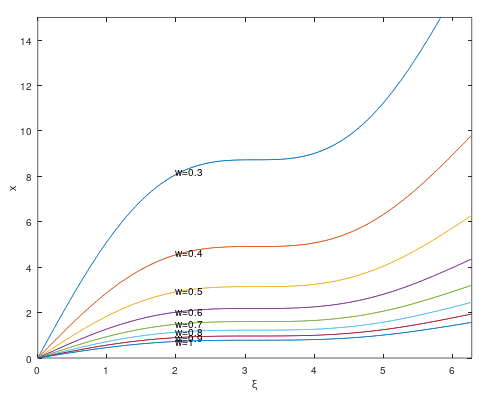
\includegraphics[width=10cm]{chapter_05_paragraph_21_exercice_6}
		\caption{Exemples de trajectoire pour diff\'erentes valeurs de fr\'equence telle que cette derni\`ere ne d\'epende pas de l'amplitude)}\label{FIG:5_21_EX6}
	\end{center}
\end{figure}

\section{Oscillations for\'ees}

Dans les excercices suivants, le syt\`eme se trouve \`a l'\'equilibre et au repos \`a l'instant $t = 0$, i.e. $x(t = 0) = 0$ et $\dot{x}(t = 0) = 0$.

\subsection{Mouvement dans le cas d'une force ext\'erieure non born\'ee dans le temps}

Il s'agit de d\'eterminer les oscillations forc\'ees, $x(t)$, d'un syst\`eme dues \`a une force $F(t)$ dans diff\'erents cas pr\'ecis.

\subsubsection{$F = F_{0}$}\label{PAR:23_EX2a}

Dans ce cas, l'\'equation (\ref{EQ:22_2}) s'\'ecrit :
\be
	\ddot{x} + \omega^{2}x = \dfrac{F_{0}}{m}
\ee
dont la solution g\'en\'erale sans second membre peut s'\'ecrire : $a\cos(\omega t + \alpha)$ et une int\'egrale particulière constante, dont la d\'eriv\'ee seconde par rapport au temps est \'evidemment nulle, telle que $\omega^{2}x = \frac{F_{0}}{m} \Leftrightarrow x = \frac{F_{0}}{m\omega^{2}}$. Les conditions initiales permettent de d\'eduire :
\be
	\begin{cases}
		\dot(x)(0) = 0 \Leftrightarrow -\frac{F_{0}}{m\omega^{2}}\omega\sin\alpha = 0 \Leftrightarrow \sin\alpha = 0 \Leftrightarrow \alpha = 0 \\
		x(0) = 0 \Leftrightarrow a + \frac{F_{0}}{m\omega^{2}} = 0
	\end{cases}
\ee
ce qui donne comme solution :
\be
	x(t) = \dfrac{F_{0}}{m\omega^{2}}(1 - \cos(\omega t))
\ee

\subsubsection{$F = at$}\label{PAR:23_EX2b}

La solution de l'\'equation (\ref{EQ:22_2}) est consiste en :
\begin{itemize}
	\item la solution g\'en\'erale sans second membre : $x_{0} = a\cos(\omega t + \alpha)$
	\item l'int\'egrale particuli\`ere : $x_{1} = bt$ qui permet d'arriver \`a : $0 + \omega^{2}bt = \frac{F_{0}}{m}t \Leftrightarrow b = \frac{F_{0}}{m\omega^{2}}$
\end{itemize}
Les condtions initialies permettent les d\'eductions suivantes :
\be
	\begin{cases}
		x(0) = 0 \Leftrightarrow \Leftrightarrow a\cos\alpha = 0 \Leftrightarrow \alpha = \pm\frac{\pi}{2} \\
		\dot{x}(0) = 0 \Leftrightarrow -a\omega\sin\alpha + \frac{F_{0}}{m\omega^{2}} = 0 \Leftrightarrow a = \pm\frac{F_{0}}{m\omega^{3}}
	\end{cases}
\ee
donc :
\be
	x(t) = \dfrac{F_{0}}{m\omega^{3}}(\omega t + \cos(\omega t \pm \pi/2)) \Leftrightarrow x(t) = \dfrac{F_{0}}{m\omega^{3}}(\omega t \pm \sin(\omega t))
\ee

\subsubsection{$F = F_{0}e^{-\alpha t}$}

Dans ce cas, l'int\'egrale particuli`ere est de la forme $be^{-\alpha t}$. En l'injectant dans l'\'equation (\ref{EQ:22_2}) :
\be
	\alpha^{2}be^{-\alpha t} + \omega^{2}be^{-\alpha t} = \dfrac{F_{0}}{m}e^{-\alpha t} \Leftrightarrow b = \dfrac{F_{0}}{m(\omega^{2} + \alpha^{2})}
\ee
ce qui permet d'\'ecrire le mouvement ainsi :
\be
	x(t) = a_{1}\cos(\omega t) + a_{2}\sin(\omega t) + \dfrac{F_{0}}{m(\omega^{2} + \alpha^{2})}e^{-\alpha t}
\ee
Les conditions initiales :
\be
	\begin{cases}
	x(t = 0) = 0 \Leftrightarrow a_{1} + \dfrac{F_{0}}{m(\omega^{2} + \alpha^{2})} = 0 \Leftrightarrow a_{1} = -\dfrac{F_{0}}{m(\omega^{2} + \alpha^{2})} \\
	\dot{x}(t = 0) = 0 \Leftrightarrow a_{2}\omega - \dfrac{F_{0}\alpha}{m(\omega^{2} + \alpha^{2})} = 0 \Leftrightarrow a_{2} = \dfrac{F_{0}\omega}{m\omega(\omega^{2} + \alpha^{2})}
	\end{cases}
\ee
permettent de conclure :
\be
	x(t) = \dfrac{F_{0}}{m(\omega^{2} + \alpha^{2})}\left(e^{-\alpha t} - \cos(\omega t) + \dfrac{\alpha}{\omega}\sin(\omega t)\right)
\ee

\begin{figure}[htb!]
	\begin{center}
		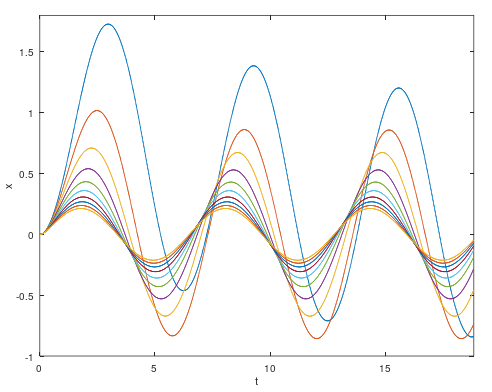
\includegraphics[width=10cm]{chapter_05_paragraph_22_exercice_1c}
		\caption{Oscillations pour $F = F_{0}e^{-\alpha t}$ et $\alpha$ de 0.1 à 5 par pas de 0.5.}\label{FIG:22_1_c}
	\end{center}
\end{figure}

\subsubsection{$F = F_{0}e^{-\alpha t}\cos\beta t$}

Dans ce cas pr\'ecis, en remarquant que $F = \Re{(\overline{F})} = \Re{(F_{0}e^{-\alpha t}e^{i\beta t})} = \Re{(F_{0}e^{(i\beta - \alpha)t})}$, nous utiliserons les formes complexes, alors :
\begin{itemize}
	\item la solution g\'n\'erale sans second membre est $\overline{x_{0}} = \overline{a}e^{i\omega t + \varphi}$
	\item l'int\'egrale particuli\`ere est $\overline{x_{1}} = \overline{b}e^{(i\beta - \alpha)t}$
\end{itemize}
avec $\{a;b\} \in \mathbb{C}$. La relation (\ref{EQ:22_2}) permet d'\'ecrire :
\bea
	\dfrac{F_{0}}{m}e^{i(\beta - \alpha)t} & = & \overline{b}(i\beta - \alpha)^{2}e^{i(\beta - \alpha)t} + \omega^{2}\overline{b}e^{i(\beta - \alpha)t} \Leftrightarrow \overline{b} = \dfrac{F_{0}}{m(\omega^{2} + (i\beta - \alpha)^{2})} \nonumber \\
	\overline{b} & = & \dfrac{F_{0}}{m(\omega^{2} - \beta^{2} + \alpha^{2} - 2i\alpha\beta)} = \dfrac{F_{0}(\omega^{2} - \beta^{2} + \alpha^{2} + 2i\alpha\beta)}{m\left((\omega^{2} - \beta^{2} + \alpha^{2})^{2} + 4\alpha^{2}\beta^{2}\right)}
\eea
La solution pour les oscillations forcées dans le domaine complexe s'\'ecrit alors en posant $a = a_{1} + ia_{2}$ avec $\{a_{2};a_{2}\} \in \mathbb{R}$ :
\bea
	\overline{x} & = & \dfrac{F_{0}(\omega^{2} - \beta^{2} + \alpha^{2} + 2i\alpha\beta)}{m\left((\omega^{2} - \beta^{2} + \alpha^{2})^{2} + 4\alpha^{2}\beta^{2}\right)}e^{(i\beta - \alpha)t}(\cos(\beta t) + i\sin(\beta t)) \nonumber \\
	& & + (a_{1} + ia_{2})\cos(\omega t) + (-a_{2} + ia_{1})\sin(\omega t)
\eea
En effet, dans la solution g\'en\'erale sans second membre, l'expression exponentielle se d\'eveloppe ainsi :
\bea
	e^{i\omega t + \varphi} & = & \cos(\omega t + \varphi) + i\sin(\omega t + \varphi) = \cos(\omega t)\cos\varphi - \sin(\omega t)\sin\varphi \nonumber \\
	& &	+ i(\cos(\omega t)\sin\varphi + \sin(\omega t)\cos\varphi) \nonumber \\
	& = & (\cos\varphi + i\sin\varphi)\cos(\omega t) + (-\sin\varphi + i\cos\varphi)\sin(\omega t)
\eea
et les facteurs $a_{1}$ et $a_{2}$ permettent de d\'efinir la phase. Ainsi :
\bea
	\overline{x} & = & a_{1}\cos(\omega t) - a_{2}\sin(\omega t) + \dfrac{F_{0}(\omega^{2} - \beta^{2} + \alpha^{2})}{m\left((\omega^{2} - \beta^{2} + \alpha^{2})^{2} \nonumber + 4\alpha^{2}\beta^{2}\right)}e^{-\alpha t}\cos(\beta t) \nonumber \\
	& & - \dfrac{2F_{0}\alpha\beta}{m\left((\omega^{2} - \beta^{2} + \alpha^{2})^{2} + 4\alpha^{2}\beta^{2}\right)}e^{-\alpha t}\sin(\beta t) \nonumber \\
	& & + i\left(a_{2}\cos(\omega t) + a_{1}\sin(\omega t) + \dfrac{F_{0}(\omega^{2} - \beta^{2} + \alpha^{2})}{m\left((\omega^{2} - \beta^{2} + \alpha^{2})^{2} + 4\alpha^{2}\beta^{2}\right)}e^{-\alpha t}\sin(\beta t) \right. \nonumber \\
	& & + \left. \dfrac{2F_{0}\alpha\beta}{m\left((\omega^{2} - \beta^{2} + \alpha^{2})^{2} + 4\alpha^{2}\beta^{2}\right)}e^{-\alpha t}\cos(\beta t)\right)
\eea
Cette expression se r\'eduit car le mouvement oscillatoire est r\'ealis\'e dans le domaine r\'eel, aussi $x = \Re{(\overline{x})}$. Les conditions initiales permettent de d\'eduire les c{\oe}fficients tels que :
\be
	x(t = 0) = 0 \Leftrightarrow a_{1} + \dfrac{F_{0}(\omega^{2} - \beta^{2} + \alpha^{2})}{m\left((\omega^{2} - \beta^{2} + \alpha^{2})^{2} + 4\alpha^{2}\beta^{2}\right)} = 0
\ee
et :
\bea
	\dot{x} & = & -a_{1}\omega\sin(\omega t) - a_{2}\omega\cos(\omega t) + \dfrac{F_{0}(\omega^{2} - \beta^{2} + \alpha^{2})}{m\left((\omega^{2} - \beta^{2} + \alpha^{2})^{2} + 4\alpha^{2}\beta^{2}\right)}\left(-\alpha e^{-\alpha t}\cos(\beta t) - \beta e^{-\alpha t}\sin(\beta t)\right)\nonumber \\
	& & - \dfrac{2F_{0}\alpha\beta}{m\left((\omega^{2} - \beta^{2} + \alpha^{2})^{2} + 4\alpha^{2}\beta^{2}\right)}\left(-\alpha e^{-\alpha t}\sin(\beta t) + \beta e^{-\alpha t}\cos(\beta t)\right)
\eea
Donc :
\bea
	0 & = & -a_{2}\omega - \dfrac{\alpha F_{0}(\omega^{2} - \beta^{2} + \alpha^{2})}{m\left((\omega^{2} - \beta^{2} + \alpha^{2})^{2} + 4\alpha^{2}\beta^{2}\right)} - \dfrac{2F_{0}\alpha\beta^{2}}{m\left((\omega^{2} - \beta^{2} + \alpha^{2})^{2} + 4\alpha^{2}\beta^{2}\right)} \nonumber \\
	\Leftrightarrow a_{2} & = & -\dfrac{\alpha F_{0}(\omega^{2} + \alpha^{2} + \beta^{2})}{m\omega\left((\omega^{2} - \beta^{2} + \alpha^{2})^{2} + 4\alpha^{2}\beta^{2}\right)}
\eea
Ainsi le mouvement est d\'ecrit par :
\bea
	x(t) & = & \dfrac{F_{0}(\omega^{2} + \alpha^{2} + \beta^{2})}{m\left((\omega^{2} - \beta^{2} + \alpha^{2})^{2} + 4\alpha^{2}\beta^{2}\right)} \left(-(\omega^{2} - \beta^{2} + \alpha^{2})\cos(\omega t) + \dfrac{\alpha}{\omega}(\omega^{2} + \alpha^{2} + \beta^{2})\sin(\omega t) \right. \nonumber \\
	& & + \left. (\omega^{2} - \beta^{2} + \alpha^{2})\cos(\beta t) -2\alpha\beta\sin(\beta t)e^{-\alpha t}\right) \\
\eea

\begin{figure}[htb!]
	\begin{center}
		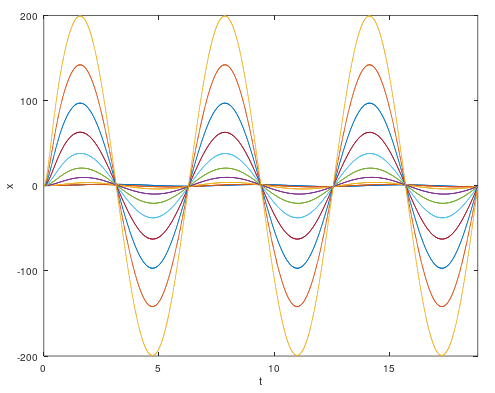
\includegraphics[width=10cm]{chapter_05_paragraph_22_exercice_1d}
		\caption{Oscillations pour $F = F_{0}e^{-\alpha t}\cos\beta t$ en supposant $\alpha = \beta$ et $\alpha$ de 1 à 5 par pas de 0.5.}\label{FIG:22_1_d}
	\end{center}
\end{figure}

\subsection{Mouvement dans le cas d'une force ext\'erieure born\'ee dans le temps}

Dans cette suite d'exercices, l'objectif est de calculer l'amplitude finale des oscillations d'un système apr\`es l'action d'une force ext\'erieure telle que $F = 0$ pour $t < 0$ et qu'\`a $t = 0$, le syt\`eme est au repos et \`a l'\'equilibre, i.e. $x(t = 0) = 0$ et $\dot{x}(t = 0) = 0$.

\subsubsection{Premier exemple}

Dans ce premier cas, la force ext\'erieure s'exprime telle que :
\begin{itemize}
	\item $F = F_{0}t/T$ pour $t \in [0;T]$
	\item $F = F_{0}$ pour $t > T$
\end{itemize}

Pour $0 < t < T$, nous pouvons repartir de la solution du probl\`eme (\ref{PAR:23_EX2b}) avec ici $a = F_{0}/T$. Aussi, nous avons dans cet intervalle de temps :
\be
	x(t) = \dfrac{F_{0}}{m\omega^{3}T}(\omega t - \sin(\omega t))
\ee
Pour $t \ge T$, c'est la solution du probl\`eme (\ref{PAR:23_EX2a}) qui peut \^etre utilis\'ee, \`a savoir $x(t) = a\cos(\omega t + \alpha) + \frac{F_{0}}{m\omega^{2}}$. Il reste \`a remplir les conditions de continuit\'e pour $t = T$, soit :
\be
	\begin{cases}
		\dfrac{F_{0}}{m\omega^{3}T}(\omega T - \sin(\omega T)) = a\cos(\omega T + \alpha) + \dfrac{F_{0}}{m\omega^{2}} \Leftrightarrow a\cos(\omega T + \alpha) = -\dfrac{F_{0}}{m\omega^{3}T}\sin(\omega T) \\
		\\
		\dfrac{F_{0}}{m\omega^{3}T}(\omega - \omega\cos(\omega T)) = -a\omega\sin(\omega T + \alpha) \Leftrightarrow a\sin(\omega T + \alpha) = \dfrac{F_{0}}{m\omega^{3}T}(1 - \cos(\omega T))
	\end{cases}
\ee
En appliquant l'identit\'e $\cos^{2} + \sin^{2} = 1$, cela permet d'en d\'eduire l'amplitude des oscillations :
\bea
	a^{2} & = & \left(-\dfrac{F_{0}}{m\omega^{3}T}\sin(\omega T)\right)^{2} + \left(\dfrac{F_{0}}{m\omega^{3}T}(1 - \cos(\omega T))\right)^{2} \nonumber \\
	& = & \left(\dfrac{F_{0}}{m\omega^{3}T}\right)^{2}\left(\sin^{2}(\omega T) + 1 + \cos^{2}(\omega T) - 2\cos(\omega T)\right) \nonumber \\
	& = & 2\left(\dfrac{F_{0}}{m\omega^{3}T}\right)^{2}(1 - \cos(\omega T)) = 4\left(\dfrac{F_{0}}{m\omega^{3}}\right)^{2}\sin^{2}\left(\dfrac{\omega T}{2}\right) \nonumber \\
	\Leftrightarrow a & = & 2\left(\dfrac{F_{0}}{m\omega^{3}T}\right)\bigg\lvert\sin\left(\dfrac{\omega T}{2}\right)\bigg\rvert
\eea

\begin{figure}[htb!]
	\begin{center}
		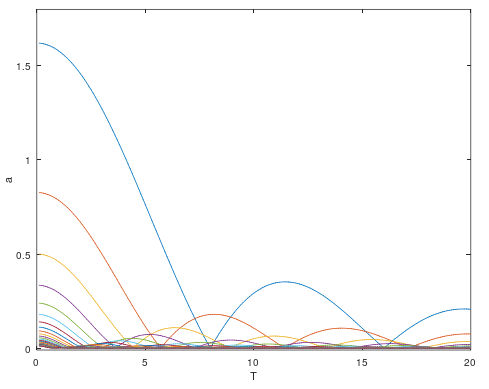
\includegraphics[width=10cm]{chapter_05_paragraph_22_exercice_2}
		\caption{\'Evolution de l'amplitude en fonction de la période pour $\omega$ de $\pi/4$ à $3\pi$}\label{FIG:22_2}
	\end{center}
\end{figure}

\subsubsection{Deuxi\`eme exemple}

Dans ce deuxi\`eme cas, la force ext\'erieure s'exprime telle que :
\begin{itemize}
	\item $F = F_{0}$ pour $t \in [0;T]$
	\item $F = 0$ pour $t > T$
\end{itemize}

La force ext\'erieure n'op\`ere plus pour $t > T$ aussi l'amplitude des oscillations au-del\`a de $T$ est exactement la valeur de l'oscillation \`a $t = T$. En reprenant la solution du probl\`eme (\ref{PAR:23_EX2a}) pour $t < T$ et appliqu\'ee en $t = T$, nous obtenons ais\'ement :
\be
	a = x(T) = \dfrac{F_{0}}{m\omega^{2}}(1 - \cos(\omega T)) = 2\dfrac{F_{0}}{m\omega^{2}}\sin^{2}\left(\dfrac{\omega T}{2}\right)
\ee
Ce r\'esultat est diff\'erent de celui pr\'esent\'e dans le livre en $\propto \sin$ au lieu de $\propto \sin^{2}$ ici obtenu.

\subsubsection{Troisi\`eme exemple}

Dans ce troisi\`eme cas, la force ext\'erieure s'exprime telle que :
\begin{itemize}
	\item $F = F_{0}t/T$ pour $t \in [0;T]$
	\item $F = 0$ pour $t > T$
\end{itemize}

Pour cet exemple, nous allons raisonner avec la variable d\'efinie en (\ref{EQ:22_9}), \`a savoir $\xi = \dot{x} + i\omega x$. Sans force ext\'erieure, i.e. pour la partie telle que $t > T$, la relation (\ref{EQ:22_10}) permet de d\'eduire l'\'energie du syst\`eme comme $\frac{1}{2}m\omega^{2}a^{2}$ alors qu'avec l'application d'une force ext\'erieure, nous avons vu par l'\'equation (\ref{EQ:22_11}) que l'\'energie du syst\`eme s'\'ecrit $\frac{1}{2}m\lvert\xi\rvert^{2}$ et en particulier $\frac{1}{2}m\lvert\xi(T)\rvert^{2}$. Comme l'\'energie du syst\`eme se conserve, nous pouvons en conclure que :
\be
	\lvert\xi(T)\rvert^{2} = \omega^{2}a^{2}
\ee
Pour $0 < t < T$, la solution du probl\`eme est celle du paragraphe (\ref{PAR:23_EX2b}) qui permet d'\'ecrire $x(t) = \frac{F_{0}}{m\omega^{3}T}(\omega t - \sin(\omega t))$. Nous avons alors :
\bea
	\xi & = & \dot{x} + i\omega x = \dfrac{F_{0}}{m\omega^{3}T}(\omega - \omega\cos(\omega t)) + i\omega\dfrac{F_{0}}{m\omega^{3}T}(\omega t - \sin(\omega t)) \nonumber \\
	& = & \dfrac{F_{0}}{m\omega^{2}T}(1 - \cos(\omega t)) + i\dfrac{F_{0}}{m\omega^{2}T}(\omega t - \sin(\omega t)) = \dfrac{F_{0}}{m\omega^{2}T}(1 - \cos(\omega t) + i(\omega t - \sin(\omega t)) \nonumber \\
	\Leftrightarrow \lvert\xi(T)\rvert^{2} & = & \dfrac{F_{0}^{2}}{m^{2}\omega^{4}T^{2}}\left((1 - \cos(\omega T)^{2} + (\omega T - \sin(\omega T))^{2}\right) \nonumber \\
	& = & \dfrac{F_{0}^{2}}{m^{2}\omega^{4}T^{2}}\left(1 + \cos^{2}(\omega T) - 2\cos(\omega T) + \omega^{2}T^{2} + \sin^{2}(\omega t) - 2\omega T\sin(\omega T)\right) \nonumber \\
	& = & \dfrac{F_{0}^{2}}{m^{2}\omega^{4}T^{2}}\left(\omega^{2}T^{2} - 2\omega T\sin(\omega T) + 2(1 - \cos(\omega T))\right)
\eea
En reprenant l'\'egalit\'e $\lvert\xi(T)\rvert^{2} = \omega^{2}a^{2}$, nous arrivons alors :
\be
	a = \dfrac{F_{0}}{m\omega^{3}T}\sqrt{\omega^{2}T^{2} - 2\omega T\sin(\omega T) + 2(1 - \cos(\omega T))}
\ee

\begin{figure}[htb!]
	\begin{center}
		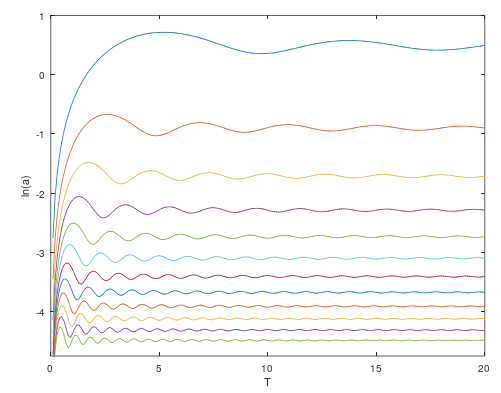
\includegraphics[width=10cm]{chapter_05_paragraph_22_exercice_4}
		\caption{\'Evolution de l'amplitude en fonction de la période pour $\omega$ de $\pi/4$ à $3\pi$}\label{FIG:22_4}
	\end{center}
\end{figure}

\subsubsection{Quatri\`eme exemple}

Dans ce dernier cas, la force ext\'erieure s'exprime telle que :
\begin{itemize}
	\item $F = F_{0}\sin(\omega t)$ pour $t \in [0;T]$
	\item $F = 0$ pour $t > T = 2\pi/\omega$
\end{itemize}
ainsi l'exercice de la force ext\'erieure ainsi que la dur\'ee d\'ependent d'ors et d\'ej\`a de la fr\'equence propre du syst\`eme. Par d\'efinition, $\sin(\omega t) = (e^{i\omega t} - e^{-i\omega t})/2i$ donc nous pouvons \'ecrire la force ext\'erieure comme $F(t) = \frac{F_{0}}{2i}(e^{i\omega t} - e^{-i\omega t})$ pour $t < T$. Les conditions initiales retenues impliquent que $\xi(t = 0) = 0$ aussi la relation (\ref{EQ:22_10}) donne :
\bea
	\xi(T) & = & \dfrac{F_{0}}{2mi}e^{i\omega T}\int_{0}^{T}\left(e^{i\omega t} - e^{-i\omega t}\right)e^{-i\omega t}\mathrm{d}t = \dfrac{F_{0}}{2mi}e^{i\omega T}\int_{0}^{T}\left(1 - e^{-2i\omega t}\right)\mathrm{d}t \nonumber \\
	& = & \dfrac{F_{0}}{2mi}e^{i\omega T}\left(T + \dfrac{1}{2i\omega}\left(e^{-2i\omega T} - 1\right)\right) = -\dfrac{F_{0}}{2m}ie^{i\omega T}\left(T - \dfrac{i}{2\omega}\left(e^{-2i\omega T} - 1\right)\right)
\eea
or $T = 2\pi/\omega$ et $\forall n \in \mathbb{Z}\text{, }e^{2in\pi} = 1$ donc :
\bea
	\xi(T) & = & -\dfrac{F_{0}}{2m}ie^{2\pi i}\left(\dfrac{2\pi}{\omega} - \dfrac{i}{2\omega}\left(e^{-4\pi i} - 1\right)\right) = -\dfrac{F_{0}\pi}{m\omega}i \nonumber \\
	\Leftrightarrow \lvert\xi(T)\rvert^{2} & = & \dfrac{F_{0}^{2}\pi^{2}}{m^{2}\omega^{2}} = a^{2}\omega^{2} \Leftrightarrow a = \dfrac{\pi F_{0}}{m\omega^{2}}
\eea

\section{Syst\`emes \`a plusieurs degr\'es de libert\'e}

\subsection{Cas d'une fonction de Lagrange donn\'ee et pour deux degr\'es de libert\'e}

L'objectif de ce probl\`eme est de d\'eterminer les oscillations du syst\`eme dont la fonction de Lagrange est :
\be
	L = \dfrac{1}{2}(\dot{x}^{2} + \dot{y}^{2}) - \dfrac{\omega_{0}^{2}}{2}(x^{2} + y^{2}) +\alpha xy
\ee
correspondant à deux syst\`emes lin\'eaires identiques de fr\'equence propre $\omega_{0}$ coupl\'es par une interaction d\'efinie par $-\alpha xy$. Les \'equations du mouvement d\'efinies par les relations (\ref{EQ:2_6}) sont :
\be
	\begin{cases}
		\dfrac{\mathrm{d}}{\mathrm{dt}}\left(\dfrac{\partial L}{\partial\dot{x}}\right) = \dfrac{\partial L}{\partial x} \Leftrightarrow \dfrac{\mathrm{d}\dot{x}}{\mathrm{dt}} = -\omega_{0}^{2}x + \alpha y \Leftrightarrow \ddot{x} + \omega_{0}^{2}x = \alpha y \\
		\\
		\dfrac{\mathrm{d}}{\mathrm{dt}}\left(\dfrac{\partial L}{\partial\dot{y}}\right) = \dfrac{\partial L}{\partial y} \Leftrightarrow \dfrac{\mathrm{d}\dot{y}}{\mathrm{dt}} = -\omega_{0}^{2}y + \alpha x \Leftrightarrow \ddot{y} + \omega_{0}^{2}y = \alpha x
	\end{cases}
\ee
En posant $x = A_{x}e^{i\omega t}$ et $y = A_{y}e^{i\omega t}$, le syst\`eme d'\'equations devient :
\be
	\begin{cases}
		-\omega^{2}A_{x} + \omega_{0}^{2}A_{x} = \alpha A_{y} \Leftrightarrow A_{x}(\omega_{0}^{2} - \omega^{2}) = \alpha A_{y} \\
		-\omega^{2}A_{y} + \omega_{0}^{2}A_{y} = \alpha A_{x} \Leftrightarrow A_{y}(\omega_{0}^{2} - \omega^{2}) = \alpha A_{x}
	\end{cases}
\ee
L'\'equation caract\'eristique est le d\'eterminant \'egal \`a 0 de la matrice correspondant au syst\`eme d'\'equations ci-dessus, soit :
\be
	(\omega_{0}^{2} - \omega^{2})^{2} - \alpha^{2} = 0 \Leftrightarrow \omega_{1}^{2} = \omega_{0}^{2} + \alpha\text{ et }\omega_{2}^{2} = \omega_{0}^{2} - \alpha
\ee
En prenant, $\omega^{2} = \omega_{1}^{2}$ nous obtenons $A_{x} = A_{y}$ alors que pour $\omega^{2} = \omega_{2}^{2}$, nous avons $A_{x} = -A_{y}$. Cela permet d'introduire les coordonn\'ees normales $Q_{1}$ et $Q_{2}$ telles que :
\be
	\begin{cases}
		x = \dfrac{1}{\sqrt{2}}(Q_{1} + Q_{2}) \\
		x = \dfrac{1}{\sqrt{2}}(Q_{1} - Q_{2})
	\end{cases}
\ee
Les c{\oe}fficients $1/\sqrt{2}$ permettent d'obtenir les c{\oe}fficient $1/2$ devant les carr\'es des vitesses dans la fonction de Lagrange du syst\`eme.

Dans le cas particulier o\`u $\alpha \ll \omega^{2}$ alors $\omega^{2} = \omega_{0}^{2} \pm \alpha = \omega_{0}^{2}(1 \pm \alpha/\omega_{0}^{2}) \approx \omega_{0}^{2}(1 \pm \alpha/(2\omega_{0}))$. Les degr\'es de libert\'e $x$ et $y$ sont l'addition de deux oscillations de fr\'equence voisine, avec un battement de $\omega_{2} - \omega_{1} = \alpha/\omega_{0}$.

\subsection{Oscillations d'un pendule double oscillant dans un plan}

Dans cet exercice, nous reprenons le pendule double introduit dans le paragraphe (\ref{PAR:5_EX1}) et illustr\'e sur la figure (\ref{FIG:1_1})) pour lequel la fonction de Lagrange du syst\`eme est :
\be
	L = \dfrac{m_{1}+m_{2}}{2}l_{1}^{2}\dot{\varphi_{1}}^{2} + \dfrac{m_{2}}{2}l_{2}^{2}\dot{\varphi_{2}}^{2} + m_{2}l_{1}l_{2}\cos(\varphi_{1} - \varphi_{2})\dot{\varphi_{1}}\dot{\varphi_{2}} + (m_{1}+m_{2})gl_{1}\cos(\varphi_{1}) + m_{2}gl_{2}\cos(\varphi_{2})
\ee
Dans le cadre des petites oscillations qui nous occupe, i.e. $\varphi_{1} \ll 1$ et $\varphi_{2} \ll 1$, la fonction de Lagrange se r\'eduit \`a :
\be
	L = \dfrac{m_{1}+m_{2}}{2}l_{1}^{2}\dot{\varphi_{1}}^{2} + \dfrac{m_{2}}{2}l_{2}^{2}\dot{\varphi_{2}}^{2} - \dfrac{(m_{1} + m_{2})}{2}gl_{1}\varphi_{1}^{2} - m_{2}gl_{2}\varphi_{2}^{2}
\ee
car $\cos\varphi \approx \cos(0) - (\varphi - 0)\sin(0) - \frac{1}{2}(\varphi - 0)^{2}\cos(0) \approx \frac{1}{2}\varphi^{2}$

\subsection{Trajectoire dans un champ central $\propto r^{2}$}\label{PAR:23_EX3}